\documentclass[a4paper]{article}
\usepackage[utf8]{inputenc}
\usepackage[spanish, es-tabla, es-noshorthands]{babel}
\usepackage[table,xcdraw]{xcolor}
\usepackage[a4paper, footnotesep = 1cm, width=20cm, top=2.5cm, height=25cm, textwidth=18cm, textheight=25cm]{geometry}
%\geometry{showframe}

\usepackage{tikz}
\usepackage{amsmath}
\usepackage{amsfonts}
\usepackage{amssymb}
\usepackage{float}
\usepackage{graphicx}
\usepackage{caption}
\usepackage{subcaption}
\usepackage{multicol}
\usepackage{multirow}
\setlength{\doublerulesep}{\arrayrulewidth}
\usepackage{booktabs}
\usepackage{mathrsfs,amsmath}
\usepackage{hyperref}
\hypersetup{
    colorlinks=true,
    linkcolor=blue,
    filecolor=magenta,      
    urlcolor=blue,
    citecolor=blue,    
}

\newcommand{\quotes}[1]{``#1''}
\usepackage{array}
\newcolumntype{C}[1]{>{\centering\let\newline\\\arraybackslash\hspace{0pt}}m{#1}}
\usepackage[american]{circuitikz}
\usetikzlibrary{calc}
\usepackage{fancyhdr}
\usepackage{units} 

\graphicspath{./Imagenes}

\pagestyle{fancy}
\fancyhf{}
\lhead{22.05 ASSD}
\rhead{Mechoulam, Lambertucci, Rodriguez, Londero}
\rfoot{Página \thepage}

\begin{document}


%Porque recurrimos a metodos de sintesis ¿No podemos grabarlo y ya?
%Explicar la idea de PSOLA y estructura interna del sonido
%Complicaciones y pitchmarks, ejemplos y resultados


\subsection{Sintesis por muestras}
La Síntesis por muestras tiene sus origines en los estudios de grabación. Previo a las técnicas de Síntesis
se debían grabar nuevamente aquellos sonidos que no satisfacían por completo a los músicos o a los ingenieros de sonido obligandolos a utilizar más horas el estudio de grabación
lo cual, por supuesto, llevaba varios gastos asociados y retrasaba la culminación del proyecto.

\subsubsection{Time Stretching}
Supongamos que deseamos grabar un comercial de televisión y por cuestiones legales debemos añadir una pequeñas aclaraciones al final del mismo. Sin embargo, el tiempo de aire es altamente costoso entonces tenemos que poder incluir toda la información necesaria en un espacio de tiempo muy pequeño. Entonces podríamos suponer que basta con grabar el mensaje a velocidad de habla normal y luego reproducirlo más rápido para que ocupe menos tiempo. Es decir reproducir el sonido salteándose segmentos para poder acortar la duración. 

\begin{figure}[H]
	\centering
	\begin{subfigure}[b]{0.4\linewidth}
		\centering
		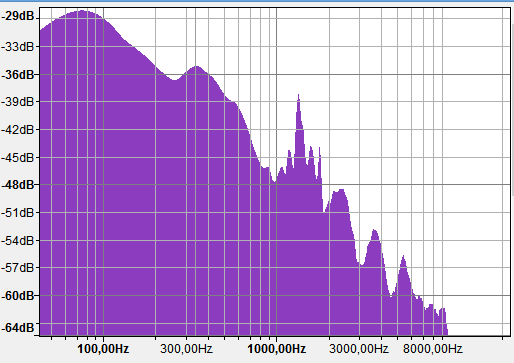
\includegraphics[scale=0.5]{ImagenesEjercicio5/HumanSpeechNormalSpeed.PNG}
		\caption{Espectro de un discurso hablado a velocidad normal}
		\label{fig:speechNormal}
	\end{subfigure}
	~
	\begin{subfigure}[b]{0.4\linewidth}
		\centering
		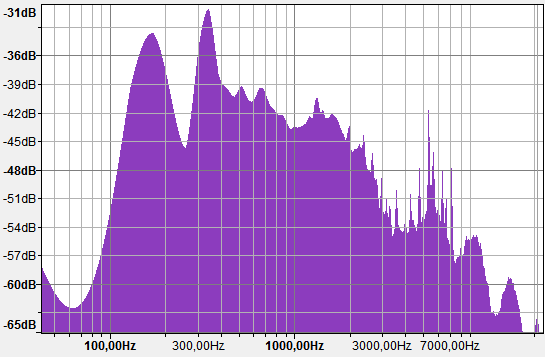
\includegraphics[scale=0.5]{ImagenesEjercicio5/HumanSpeech4X.PNG}
		\caption{Espectro del discurso con una velocidad 4 veces mayor}
		\label{fig:speech4X}
	\end{subfigure}
	\caption{Consecuencias de la compresión temporal}
\end{figure}

Como se puede observar, la figura \ref{fig:speechNormal} representa el espectro de habla de una persona hablando a una velocidad promedio. Notamos que la zona de mayor contenido armónico se halla dentro aproximadamente entre los $80Hz$ y $200Hz$. Sin embargo, si miramos al espectro del mismo discurso pero de duración 4 veces,figura \ref{fig:speech4X} menor podemos observar que el espectro no se preservo. De hecho se puede notar que hay mayor potencia espectral a frecuencias más altas que en el espectro original. Esto se traduce en un sonido chillón que poco nos recuerda al discurso original. Entonces ¿Como conseguir un sonido de menor duración pero sin distorsionar el espectro original?


\subsubsection{PSOLA}
\textbf{PSOLA} son las siglas para Pitch-Synchronus Overlap Add.



\subsubsection{Pitch Marks}
Los \textbf{pitch marks} representan momentos del sonido en el que su amplitud es máxima en un entorno. Estos puntos son los puntos centrales de la estructura del sonido. Poder localizarlos con precisión son un punto clave para los algoritmos que se basan en ellos para sintetizar nuevos sonidos.
\begin{figure}[H]
	\centering
	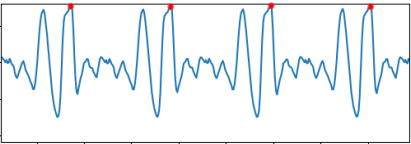
\includegraphics[width=0.7\linewidth]{ImagenesEjercicio5/soundZoomPMS.PNG}
	\caption{Imagen aumentada de una nota musical}
	\label{fig:soundzoom}
\end{figure}



 











\end{document}